\documentclass{article}

\usepackage[utf8]{inputenc}

\usepackage{graphicx}
\graphicspath{ {./Resources/} }

\title{ConOps - Inverted Pendulum PID Controller}       % Title
\author{Austin, Joe, Matt, Kathryn}                     % Team members
% \institute{SNHU/CETA}                                   % Institute
% \logo{
\includegraphics[height=0.8cm]{../../AJMK_Logo}}  % Our Logo

\begin{document}

\maketitle % Draw the title page


\section{Stakeholders}

Stakeholders are the people and organizations who have a stake or say in the actual
implementation and review of our proposed system, these include:

\begin{itemize}
    \item Educators and Acedemics,
    \item Industrial Training
    \item Producers of parts and service
\end{itemize}


\section{System Description}

A PID system is a general method for a computer or intelligent system to reduce the error
or deviation in a system. Examples include the thermostat in a stove, the cruise control in a
car or the gain control on a phone microphone.

This system aims to help display the fundamentals of a PID system in the form of a machine dedicated
to allowing the operator to experiment with the tuning and functions behind the algorithm.

It will be constructed from steel and wood, powered by a single motor and a small processor
and power supply, portable but robust enough to be installed in semi-permanent use.
Weighing between 40 and 70lb, with a tft screen. The system will use a demo PID loop to
balance an inverted pendulum and allow user input to control the rates and response of the loop.


\section{Operational Environment}

This demonstrator will be in a:

\begin{itemize}
    \item High traffic environment
    \item Possibly dusty
    \item Indoors
    \item Powered on 24/7
\end{itemize}

The enviorment the unit is placed in will affect the Support Enviorment.


\section{Support Environment}

This demonstrator will be made from as many COTS (Common Off The Shelf) parts
as possible to ensure simple replacement.

The enviorment the unit is in will affect many parts of this demonstrator

\begin{itemize}
    \item Wearing components (belts, sliders)
    \item[Mitigation] All wearable parts will be accesable and removable without major dissasembly.
    \item Constant touching and interaction
    \item[Mitigation] The demonstrator will be built from sturdy and easy to clean components.
    \item Constant uptime
    \item[Mitigation] Low power/sleep mode can prolong the life of electronics when not in use
\end{itemize}

Anything requiring major dissasembly, prolonged repair or specailaty parts will be built robust and
within manufacturer spec with documentation alongside. All systems either self calibrating or
not requiring calibration. The system will be designed with long life servicibility in mind.


\section{Operating Modes}
% Operating modes goes here

\begin{itemize}
    \item Off mode: the state in which the system is powered down and or unplugged.
    \item Idle mode: a power saving mode in which fans are turned off; the TFT screen is turned off; and the motor controller, CPU, and power supply will be swapped to their internal lower power consumption mode.
    \item Spin-up mode: a custom control procedure that self initializes (swing the pendulum up into a ready state using harmonic oscillation.
    \item Demo PID mode: a build-in PID procedure with lock Kp, Ki, and Kd values to demonstrate how the inverse pendulum is properly balanced.
    \item User PID mode: a control structure in which the user can manipulate the Kp, Ki, and Kd constants to witness the effects of their changes on the stability of the pendulum.
\end{itemize}


\section{Use}

This system will provide an excellend robust teaching tool for its users to grasp and deeply
understand the function of a PID loop, witch is an essential software and hardware algorithm
for many industries.


\section{Risks}

This system introduces risks

\begin{tabular}{ |p{1.5cm}|p{1.5cm}||p{3cm}|p{6cm}|  }
    \hline
    Likelyhood & Severity & Risk                                       & Mitigation           \\
    \hline
    10         & 8        & Pinch Points and swinging pendulum         & Capacitive e-stop
    technology as well as sound alerts when the system begins to move, and a
    transparent shield / cover to isolate the dynamic system.                                 \\
    \hline
    2          & 5        & Failure in-situ                            & Easily serviceable
    parts.
    \\
    \hline
    2          & 2        & Damaged to the unit from normal use        & Software locks, an
    e-stop switch, and a rubber bumper / mechanical hard stops.
    \\
    \hline
    1          & 5        & Short circuits and electrical malfunctions & Have a fused power
    supply, and will follow IEC standards with proper grounding.
    \\
    \hline
    3          & 5        & Heat                                       & Embedded fans in the
    storage with plenty of holes for ventilation.
    \\
    \hline
\end{tabular}


\section{Impact Considerations}

There are some considerations to think about with the implementation of this
sytem, such as

\begin{itemize}
    \item Being a hazzard and risking misuse.
    \item Requiring physical space, either for storage or use.
    \item Producing a significant amount of polutant to construct, deploy, and
          eventually recycle/throw away.
\end{itemize}


\pagebreak
\section{Inital Renders}
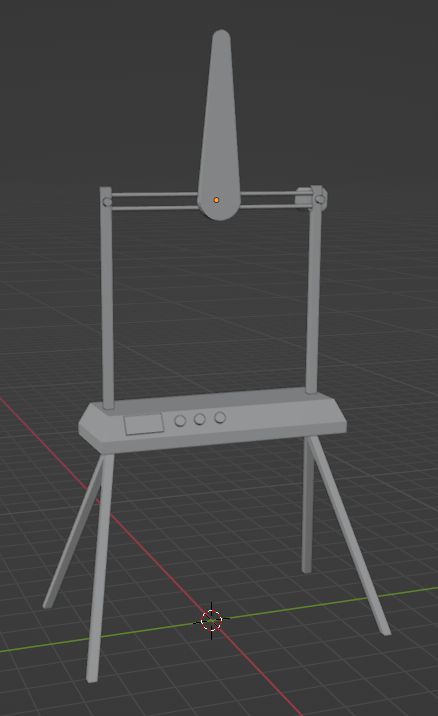
\includegraphics[height=7cm]{Full}

\vspace{1cm}

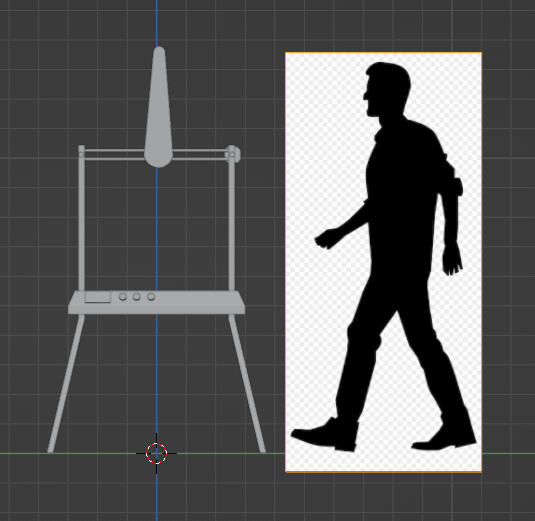
\includegraphics[width=5cm]{Scale}

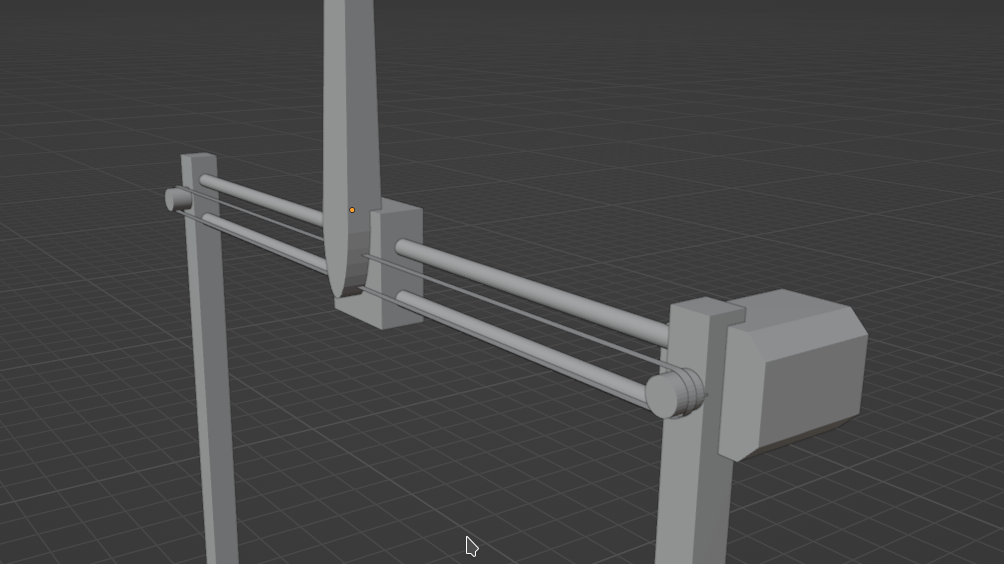
\includegraphics[width=5cm]{UpperAssy}
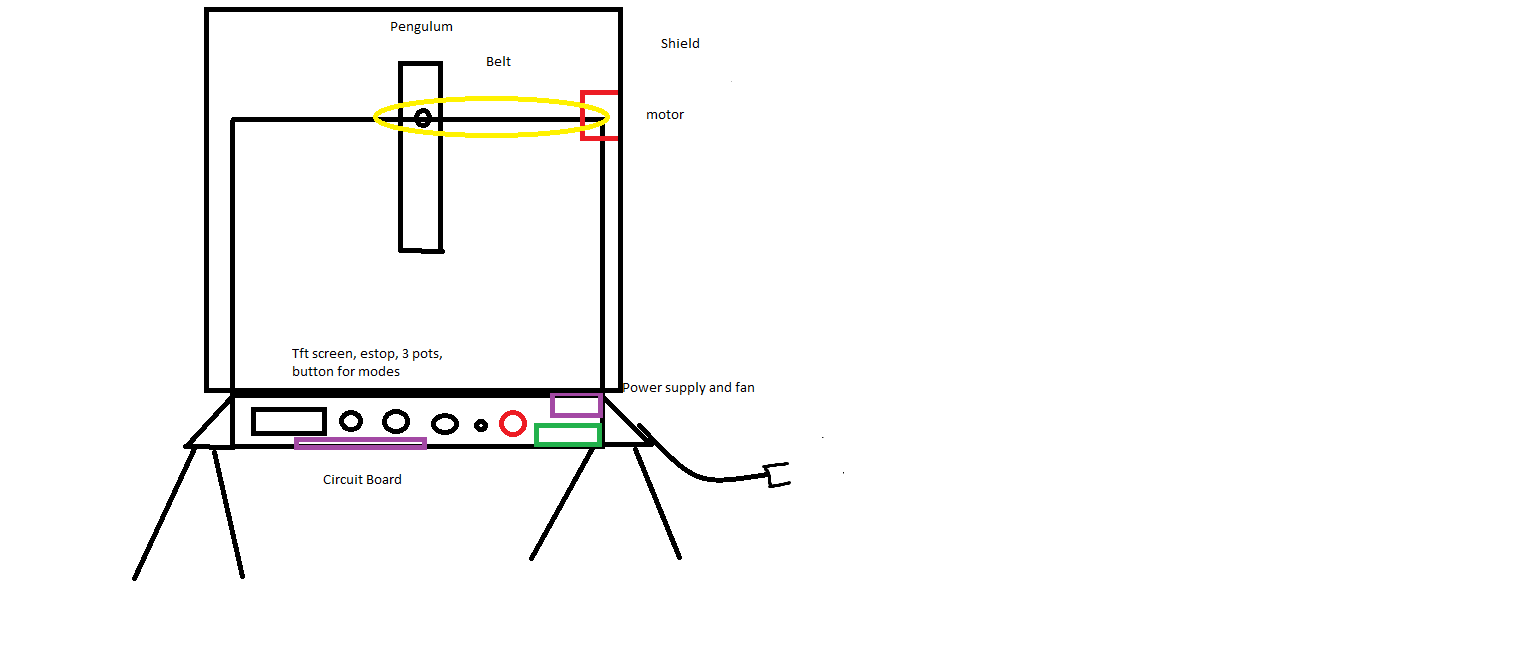
\includegraphics[width=7cm]{../../Notes/Sketches/Basic Mock-Up Sketch.png}

\vspace{1cm}
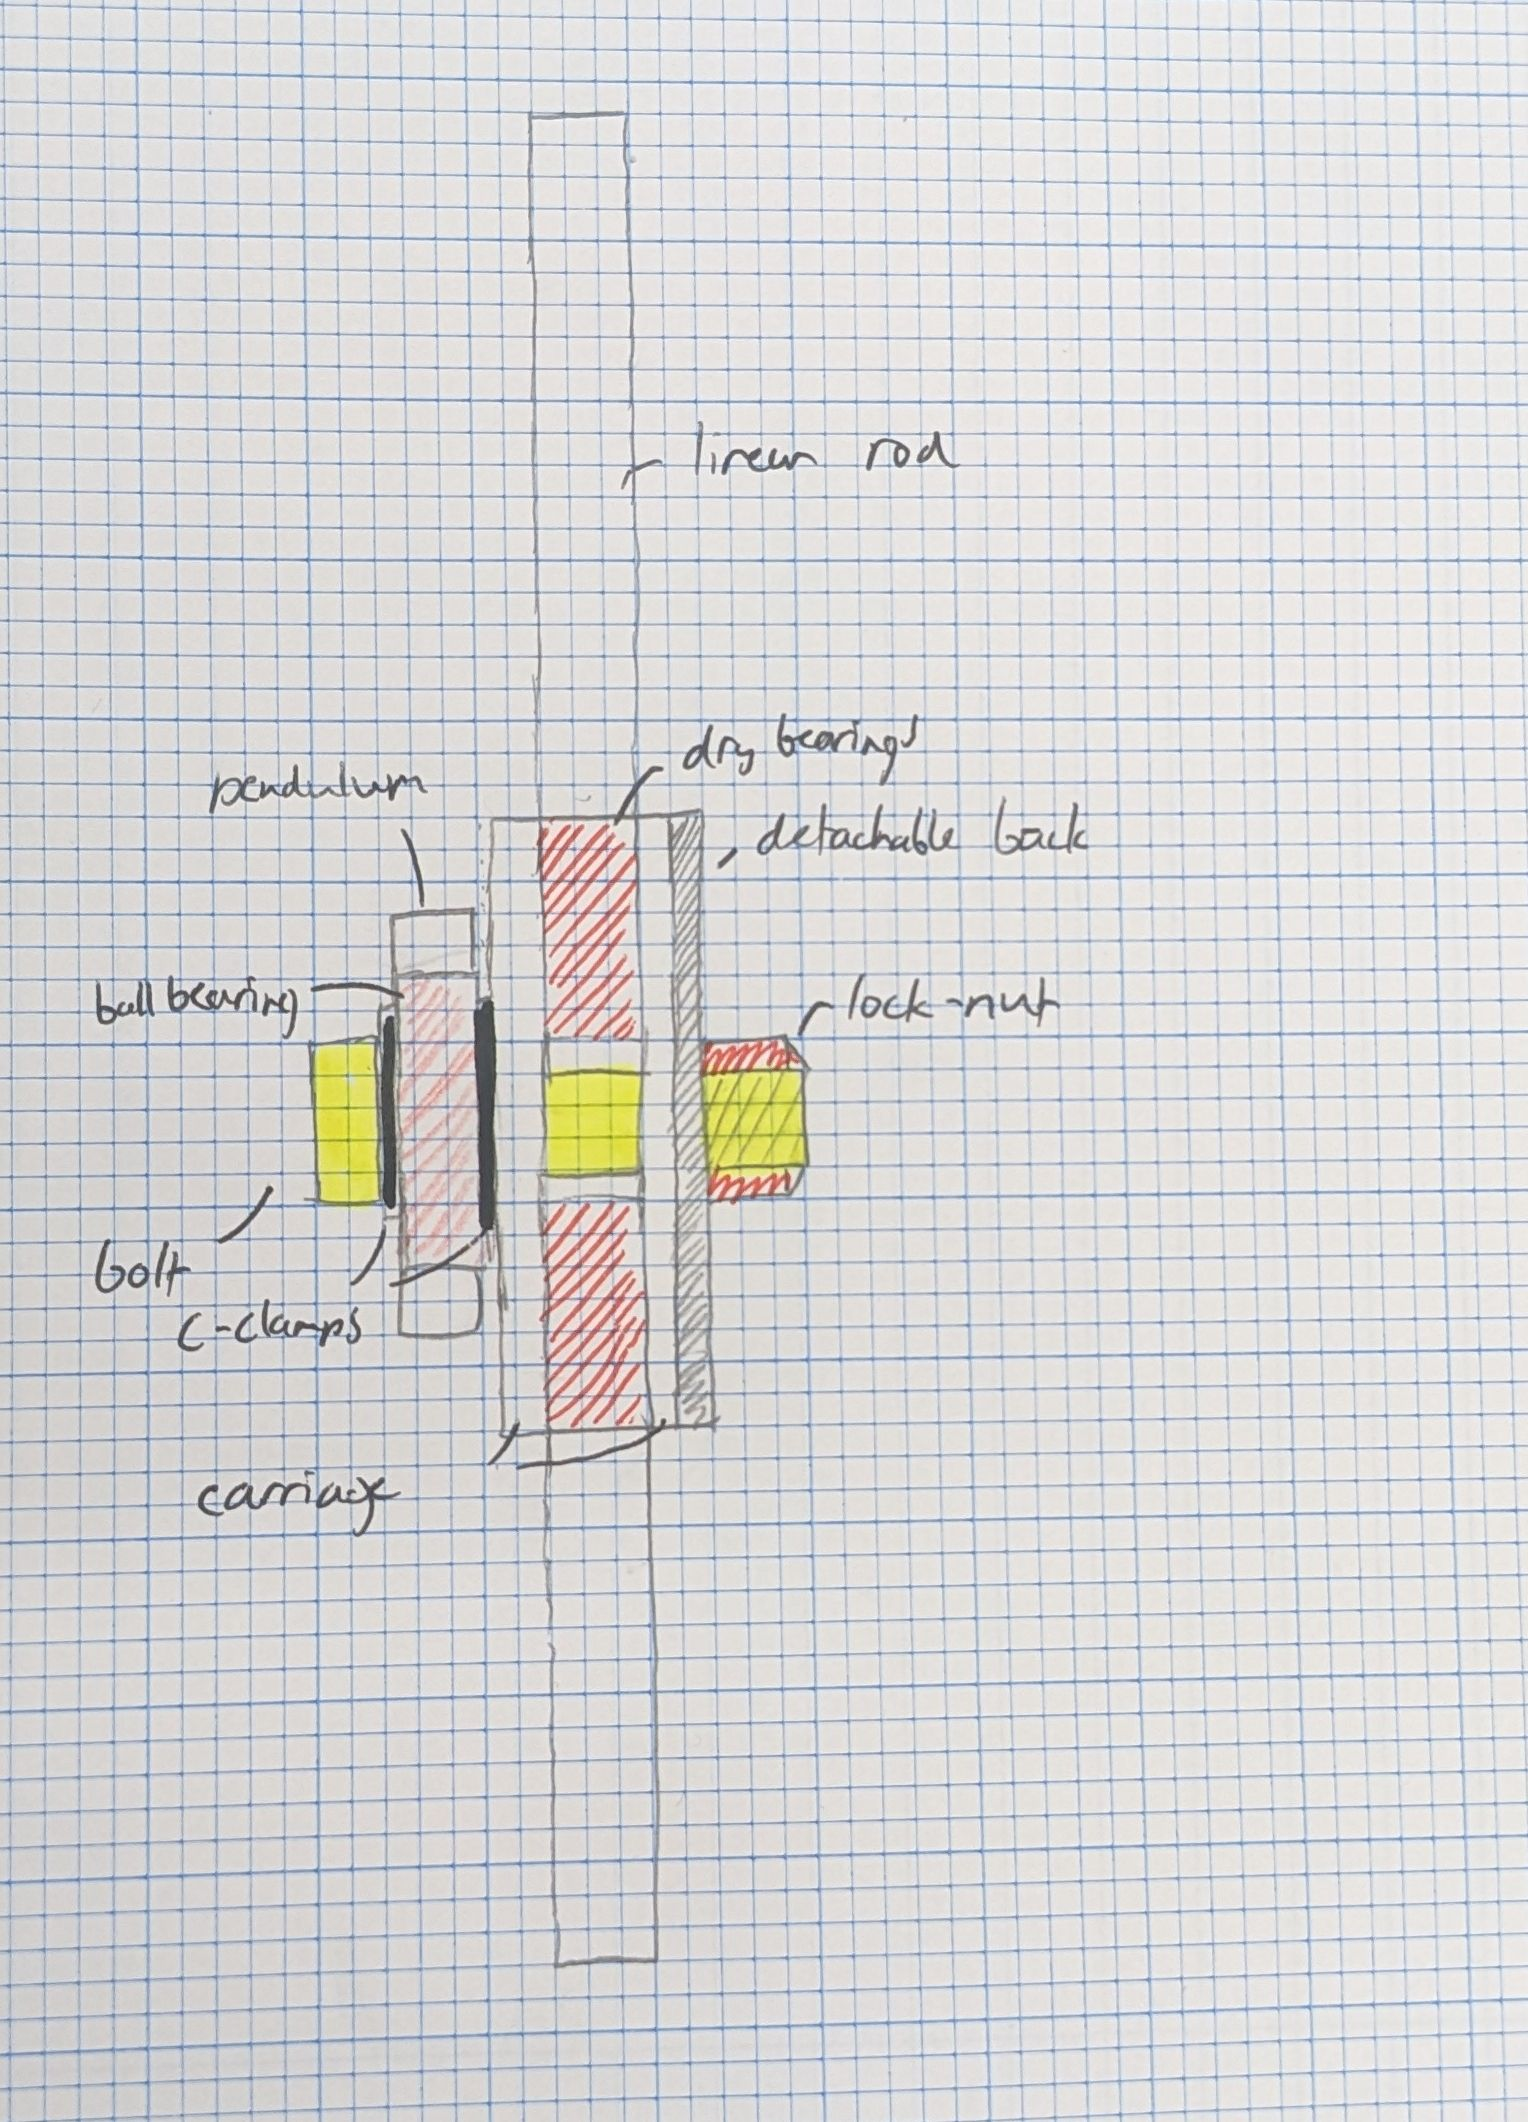
\includegraphics[height=7cm]{../../Notes/Sketches/BearingStackup.jpg}

\end{document}
